\documentclass{standalone}
\usepackage{diplomski}

\begin{document}

\chapter{Discussion and enhancements} \label{ch:discussion}
\pagenumbering{arabic}
\setcounter{page}\thestranica

% --------------------------------------

The implemented system produced a fine temperature and spatial resolution. Some issues that were discussed could be mitigated by hardware or software enhancements. Firstly, measurement fibres should be properly terminated, and the use of opto-mechanical connectors reduced. Connectors, especially those of FC-type, have demonstrated large reflections, that can even induce the occurrence of SRS at otherwise moderate optical powers. Therefore, splicing of all fibre sections is recommended. This ensures very small insertion losses, as was evident by the results represented in chapter \ref{ch:results}. \\

The used laser source proved to be sufficient in obtaining good measurement results in this system. It was, however, noted that the laser did not feature any power control, and that once configured power levels were unrepeatable and unstable during a measurement period. This phenomenon has little effect on measurement performance, as the Stokes and anti-Stokes signal, both influenced by incident optical power change, are divided in the numerical process. As long as the fibre remains in the spontaneous-Raman regime, laser instability will be negligible. Laser pulse was, however, noted to be of irregular shape, having two significant peaks, as presented in Figure \ref{fig:laser_waveform}.
\begin{figure}[h]
	\centering
	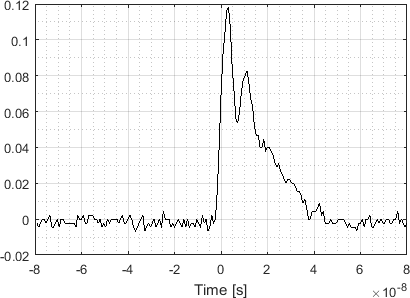
\includegraphics[width=0.8\textwidth]{laser_waveform.png}
	\caption{Laser impulse waveform, $T_0 = \SI{25}{\nano \second}$}
	\label{fig:laser_waveform}
\end{figure}
The theoretical background assumes a step-like optical excitation of the measurement fibre. Therefore, an excitation by any other waveform will in fact produce a convolution of the impulse waveform $l(t)$ with the system impulse response $h(t)$, as
\begin{equation}
y(t) = l(t) \ast h(t) \textrm{.}
\end{equation}
In situations where the laser pulse is extremely malformed, it is advisable to perform deconvolution an re-convolution with a step excitation
\begin{equation}
s(t) = \mu(t) - \mu(t-T) \textrm{,}
\end{equation}
where $\mu(t)$ is the elementary step signal. After re-convolving, we arrive at fibre measurement system step response
\begin{equation}
r(t) = s(t) \ast h(t) \textrm{.}
\end{equation}
Here, the length $T$ of step signal $s(t)$ matches the configured laser pulse width. The impulse response $h(t)$ can be found by some of the deconvolution algorithms \cite{fer:obrinf}. Here, a Fast-Fourier-transform-based (abbr. FFT) algorithm was used to apply the suggested procedure and determine the effect of the irregular laser pulse. The transfer function $H(j\omega)$ of the measurement fibre was found as a ratio of Fourier transforms of the measured laser pulse and system response
\begin{equation}
H(j\omega) = \frac{Y(j\omega)}{L(j\omega)} \textrm{.}
\end{equation}
The impulse response was then calculated as the inverse FFT and convolved by $s(t)$. The procedure, however, required very large memory resources, and was questioned to have large influence on the final measurement, in comparison to photodetectors' bandwidth issues. Therefore, after some tests that proved no significant difference would be made, the correction was concluded to be unnecessary, and scrapped. \\

Limitations on the data acquisition rate, considering the rate of data transfer between the DAQ card and the acquisition software, and not the sampling rate itself, have already been emphasised in chapter \ref{ch:results}. Better acquisition mechanism should be implemented. The first suggestion is to abandon the use of Express VIs, which may be poorly optimized, although they provide a user-friendlier configuration interface. Use of classic LabVIEW blocks may provide better overall performance. \\

Still addressing the acquisition repetition rate, some methods employing pulse coding and laser modulation have been suggested. Papers addressing this method suggest repeating the excitation pulse in a short time-period, causing an \textit{overlap} between optical pulses and their backscatterings within the measurement fibre \cite{coding1}\cite{coding2}. An example of such a method is modulating the laser with an amplitude-shift-keyed (abbr. ASK) message to obtain an effective convolution of the backscattered signals, as
\begin{equation}
y(t) = \sum_{i = 0}^{N-1} a_i x(t - iT) \textrm{,}
\end{equation}
where $x(t)$ is a single-pulsed response, and $y(t)$ the total response. The resulting signal can be numerically processed to obtain $x(t)$. Coding gain of the method can be obtained as a ratio of standard deviations of $y(t)$ and $x(t)$.
\begin{equation}
C_\textrm{gain} = \frac{\sigma_Y}{\sigma_X} = \frac{N+1}{2 \sqrt{N}}
\end{equation}
The laser used in this setup is capable of receiving an external trigger in the range of 100 Hz -- 1 MHz, which is too low a repetition rate to achieve high coding gain. Additionally, the National Instruments PXIe-1082-based system had no fast digital outputs at the time of considering this method, so producing a synchronized high-bit-rate ASK-coded message required additional hardware solutions. Therefore, this method was not implemented. \\

The next logical step towards improving the SNR of the measurement system is implementing an APD-based photodetector on Stokes channel, as well the anti-Stokes channel. SNR improvement after implementing the first diode was evident, and a very large bandwidth was able to visibly compensate for insufficiencies on the Stokes channel. Large bandwidth is desirable to detect any kinds of temperature changes, especially those occurring in a short fibre section.

% --------------------------------------

\setcounter{stranica}{\thepage}
\addtocounter{stranica}{1}

\end{document}